\documentclass[12pt,a4paper]{article}
\usepackage{physics}
\usepackage{amssymb}
\usepackage{subcaption}
\usepackage{colortbl}
\usepackage{musicography}
\newcommand{\activity}{Activity 9 -- Playing notes by image processing}
\input{spp.dat}

\begin{document}

\title{\TitleFont \activity}
\author[ ]{\textbf{Kenneth V. Domingo} \\
2015--03116 \\
App Physics 186, 1\textsuperscript{st} Semester, A.Y. 2019--20}
\affil[ ]{\corremail{kvdomingo@up.edu.ph} }

\maketitle
\thispagestyle{titlestyle}

\section*{Results and Discussion}
\setcounter{section}{1}
For this activity \cite{soriano}, I recreated the tapping part of Tom's Story's ``Anchors'' using Guitar Pro and exported it as a \texttt{png}. The excerpt is shown in Fig. \ref{fig:anchors1}. Notice that the song is in the key of G, as denoted by the sharp accidental next to the treble clef. This sort of makes things easier as we won't have to worry about accidentals in the rest of the sheet, but this only works assuming that there are no borrowed chords or if we work strictly within the major mode. The methodology I will be following is based on \cite{harris}, with some inspiration from \cite{romero} and \cite{medrana}.

\begin{figure}[htb]
	\centering
	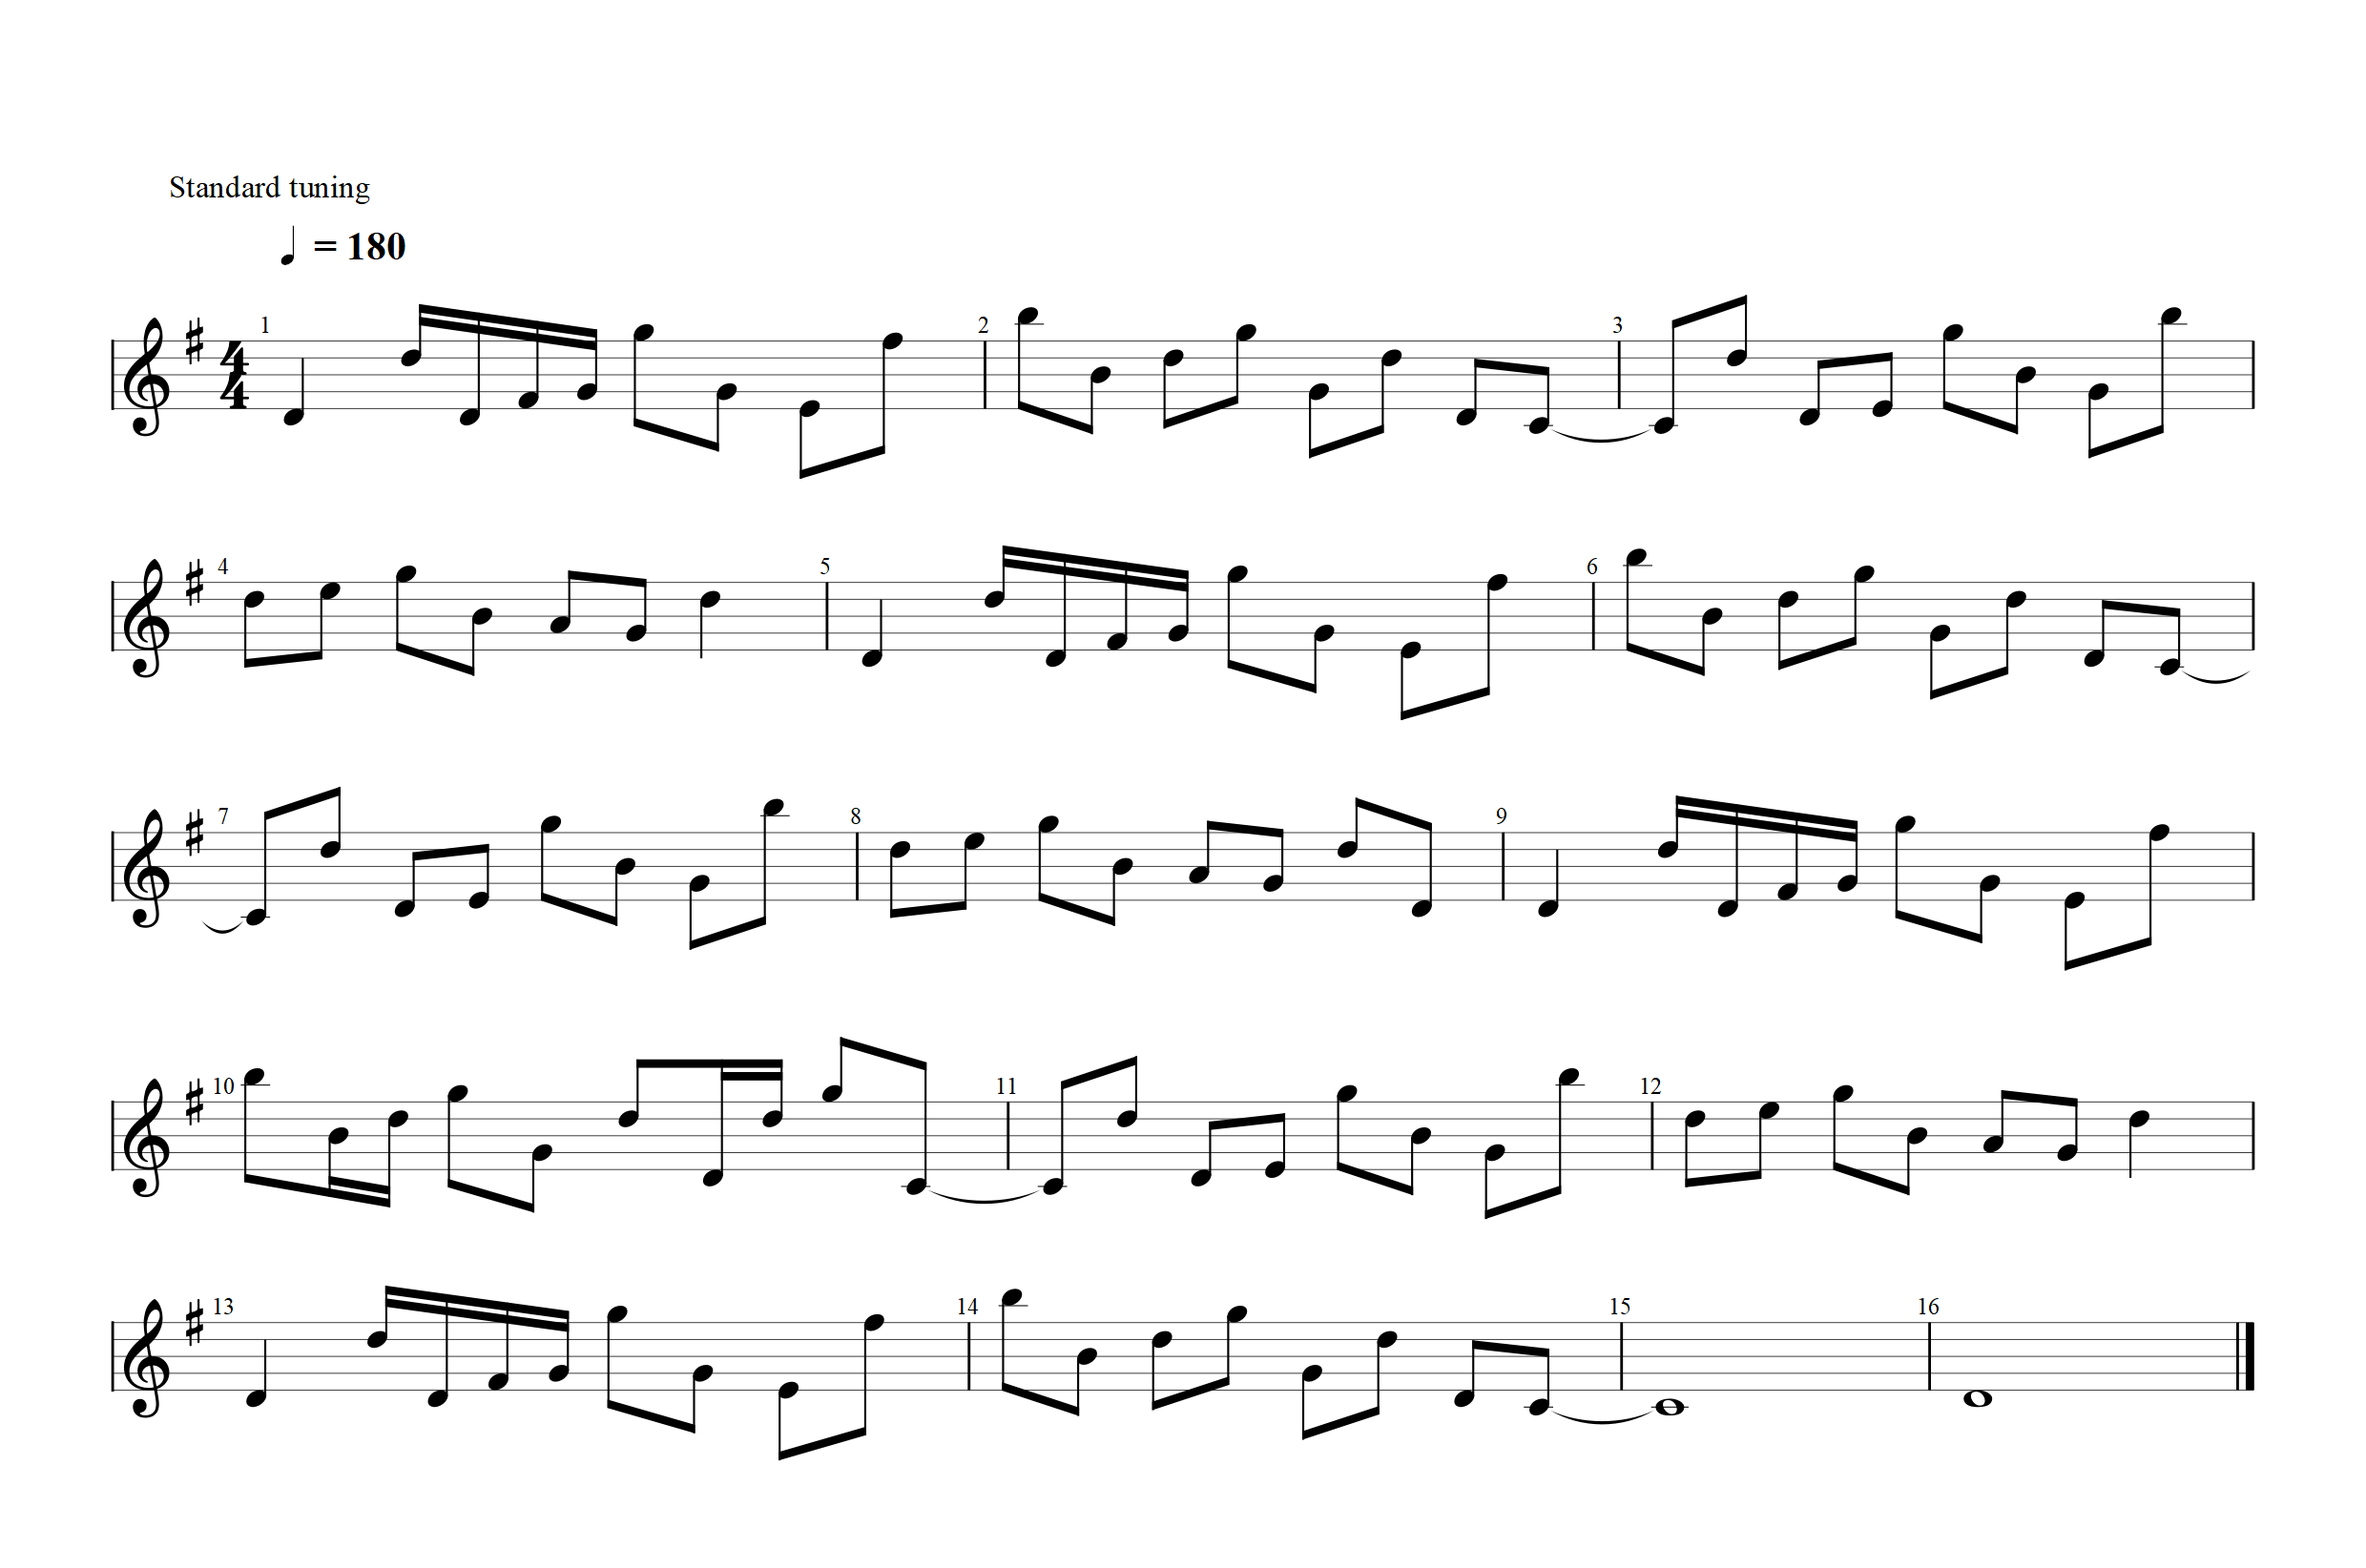
\includegraphics[width=\textwidth]{anc_truncated.png}
	\caption{Tapping portion of ``Anchors'' by Tom's Story.}
	\label{fig:anchors1}
\end{figure}

\subsection{Pre-processing}
First, the image is binarized using Otsu's method. The full track consists of 5 rows, so the image is first separated by row. This is achieved by searching for blocks with high variation and minimum vertical size \cite{vangent}. The location of the staff lines can be obtained by projecting the image onto the $y$-axis; the staff lines show up as five distinct peaks. After obtaining their index locations using Python's \texttt{peakutils} library, the staff lines can be removed by using an opening morphological operator with a horizontal line. The result of this operation is shown in Fig. \ref{fig:anc-nolines}.

\begin{figure}[htb]
	\centering
	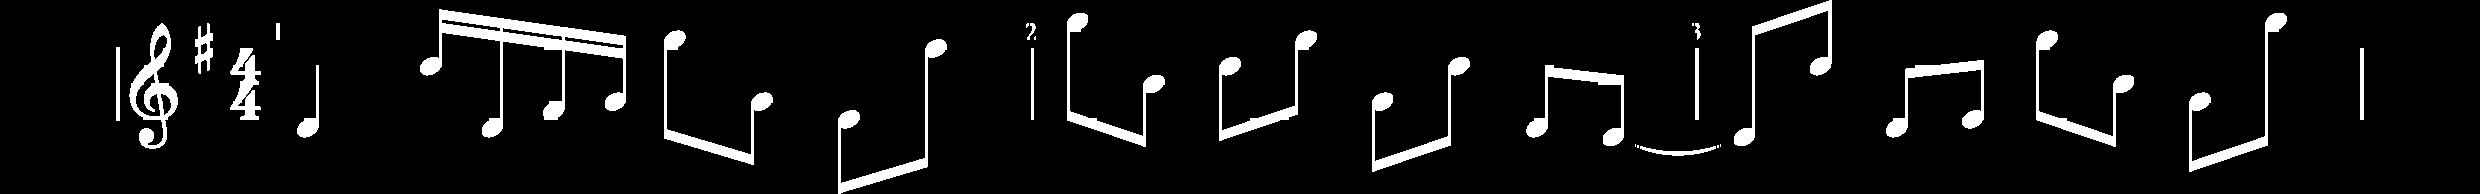
\includegraphics[width=\textwidth]{anc_nolines.png}
	\caption{First row, binarized with staff lines removed.}
	\label{fig:anc-nolines}
\end{figure}

\subsection{Object detection}
The quarter, eighth, and sixteenth notes can easily be detected because their common denominator is their filled ellipsoid bodies. Telling them apart will depend on their connection to adjacent notes (or lack thereof). To do this, the image is eroded by a vertical line so that only the note body and horizontal stems remain (Fig. \ref{fig:anc-cutstems}). Next, the location of the note bodies are obtained by further eroding the image using an ellipse kernel and using the Determinant of Hessian blob detection algorithm from the \texttt{skimage} library (Fig. \ref{fig:anc-notebodies}). We then go back to the prior image and scan the entire column spanned by one blob. If a large peak is detected, then the note is classified as an eighth. If two peaks are detected, then the classification is a sixteenth. If no other features are detected, the classification is quarter.

Whole and half notes are detected by detecting the location of regions enclosing an empty space using watershed algorithm \cite{bieniek}. Similarly, we can tell apart whole and half notes by scanning the columns spanned by the note and looking for other features.

Other features such as dotted notes and rests will not be detected.

\begin{figure}[htb]
	\centering
	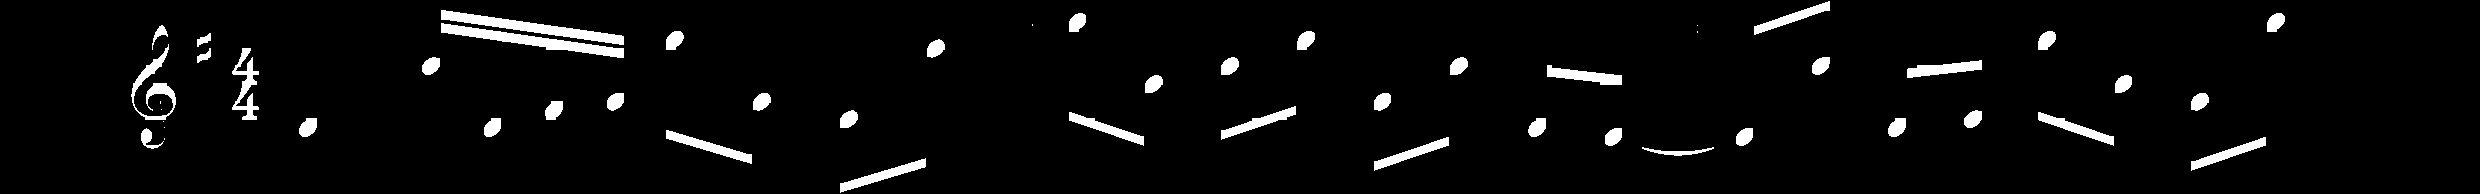
\includegraphics[width=\textwidth]{anc_cutstem.png}
	\caption{First row with eroded vertical stems.}
	\label{fig:anc-cutstems}
\end{figure}

\begin{figure}[htb]
	\centering
	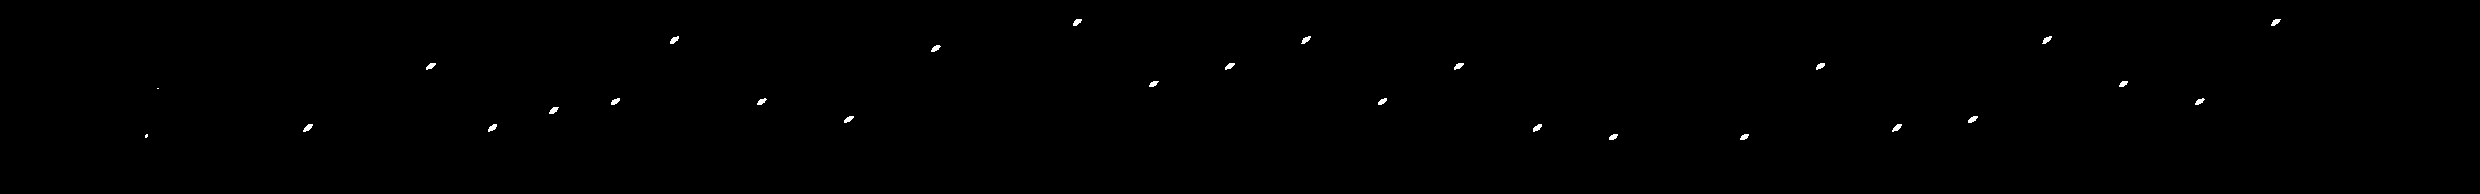
\includegraphics[width=\textwidth]{anc_notebodies.png}
	\caption{First row with only the note bodies.}
	\label{fig:anc-notebodies}
\end{figure}

\subsection{Audio synthesis}
For this section, I used the \texttt{midiutil} library to generate and save the notes as a \texttt{midi} file. Earlier, we saved the locations of the staff lines. We can use this to calculate the thickness of the staff lines and the spacing between them in pixels, which are more or less equal. We define standard A (A$_5$) to be 440 Hz, such that middle A (A$_4$) is 220 Hz. From there, we can determine the frequency of every other note by incrementing by a factor of $\sqrt[12]{2}$, assuming equal temperament. Since we are in the major mode of G, the note intervals are defined by W-W-H-W-W-W-H, which gives us the heptatonic sequence G-A-B-C-D-E-F\sh{}. For easy reference, we set our origin to be G$_4$ (second staff line), with a frequency of 196 Hz. In order to know the duration of one note, the sheet defines one quarter note to be 180 bpm, i.e., 0.33 seconds per quarter note. Instead of storing a lookup table for each note, we store instead the note intervals defined earlier whether we are jumping a whole step or a half step ($\times \sqrt[12]{2}$ or $\times \sqrt[6]{2}$, respectively) based on the number of lines (or spaces) away from middle G. With this, coupled with the note duration, we are ready to generate our audio. The \texttt{MIDIFile} function renders notes as if they were played on a piano. The final render can be accessed via \url{https://drive.google.com/open?id=11aks0IiNcZTAsTAgSVODbeYYmv8XWWPF}. The file can be played using Windows Media Player (on Windows).


\clearpage
\begin{table}[!htb]
	\centering
	\caption{Self-evaluation.}
	\begin{tabular}{||r|c||}
		\hline
		Technical correctness & 4 \\ \hline
		Quality of presentation & 5 \\ \hline
		Initiative & 0 \\ \hline
		\textbf{TOTAL} & \textbf{9} \\ \hline
	\end{tabular}
	\label{tab:self-eval}
\end{table}

\bibliographystyle{spp-bst}
\bibliography{biblio}

\end{document}